\section{Definition}

The $n=2$ \textit{n}-vector model is the one of interest in this treatment and 
it is the so called \emph{XY model}. The name is due to the fact that the spin 
is a two dimensional vector lying on the xy plane. Introduced in the 1950s, 
this model was actually used to describe quantum lattice gas and superfluid 
transitions, then in the late 1960s it was adopted to model ferromagnets.

As in any \textit{n}-vector model properties of the system are detrmined also
by the dimensionality of the lattice considered to describe the system. In the 1 
dimensional case there exists an exact solution in the absence of an external
field. Being exactly solvable means an exact form for the partition function can
be found and thermodinamical properties can be derived theoretically. When 
periodic boundaries conditions are applied, using the statistical mechanics 
\emph{transfer-matrix method}, first introduced by Kramers and Winnier in the
study of the Ising model in 1941\footnote{see \cite{Kramers1941}}, the 
partition function can be written in a very simple form as 
\begin{equation}
\label{eq:part1d}
Z = 2\pi I_0(\beta J)
\end{equation}
where $I_0(x)$ is the first modified Bessel function and $\beta = 1/k_B T$.
From equation~\ref{eq:part1d} the specific heat, and other thermodinamical 
quantities, can be exactly derived and is plotted in figure~\ref{fig:1D_XY} below.
\footnote{source 
\url{https://upload.wikimedia.org/wikipedia/commons/6/68/1D_XY_Specific_Heat.svg}} 

\begin{figure}
\label{fig:1D_XY}
\centering
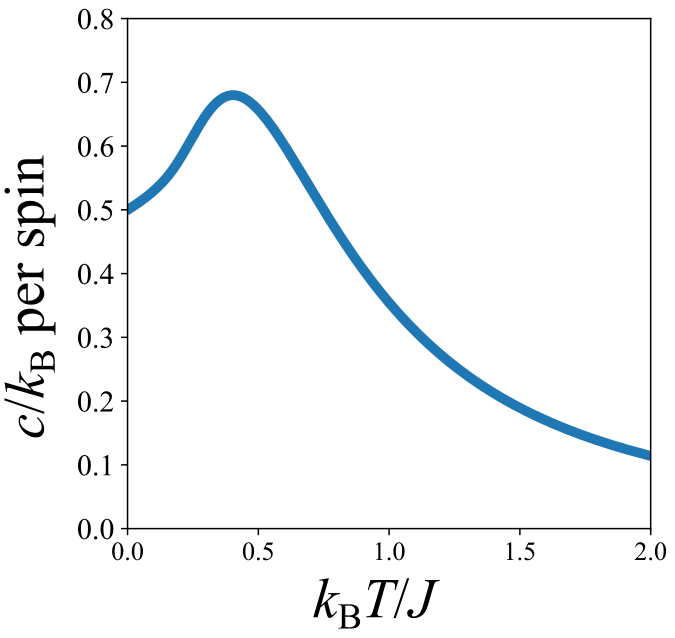
\includegraphics[scale=0.33]{1D_XY_Cv.png}
\caption{Exact specific heat of 1D XY model}
\end{figure}

The most physically interesting cases are the 2 dimensional and the 3 dimensional
one and they will be discussed in detais in the following sections.


\section{2D case}


% \section{Kosterlitz–Thouless transition}


\section{3D case}


